% Options for packages loaded elsewhere
\PassOptionsToPackage{unicode}{hyperref}
\PassOptionsToPackage{hyphens}{url}
%
\documentclass[
  ignorenonframetext,
]{beamer}
\usebackgroundtemplate{%
  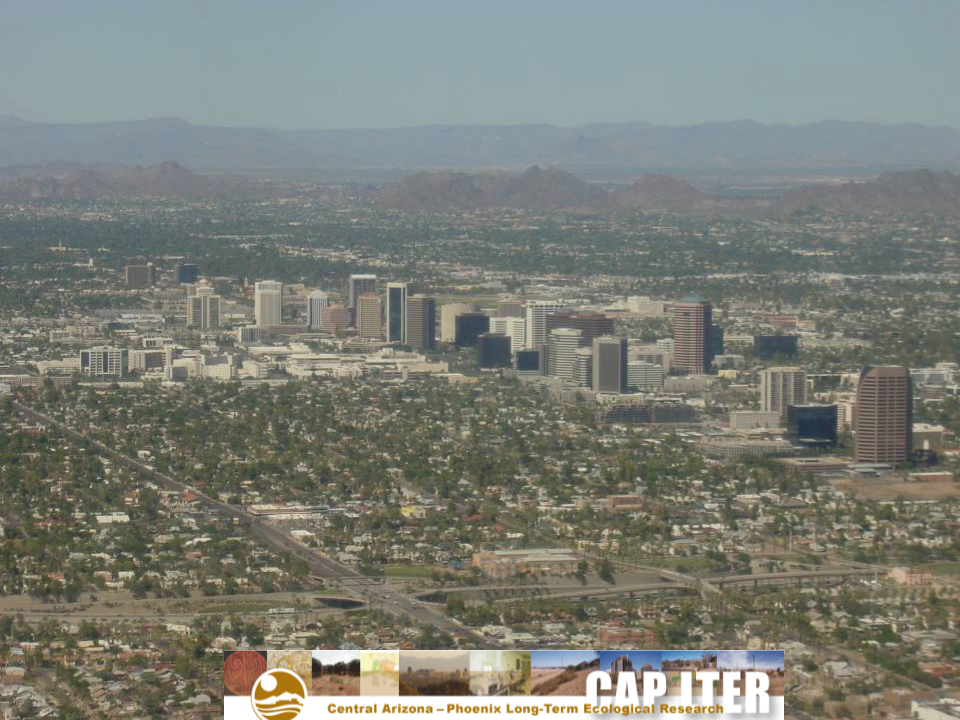
\includegraphics[width=\paperwidth]{url(assets/figures/cap-background.png)}%
}
\usepackage{pgfpages}
\setbeamertemplate{caption}[numbered]
\setbeamertemplate{caption label separator}{: }
\setbeamercolor{caption name}{fg=normal text.fg}
\beamertemplatenavigationsymbolsempty
% Prevent slide breaks in the middle of a paragraph
\widowpenalties 1 10000
\raggedbottom
\setbeamertemplate{part page}{
  \centering
  \begin{beamercolorbox}[sep=16pt,center]{part title}
    \usebeamerfont{part title}\insertpart\par
  \end{beamercolorbox}
}
\setbeamertemplate{section page}{
  \centering
  \begin{beamercolorbox}[sep=12pt,center]{part title}
    \usebeamerfont{section title}\insertsection\par
  \end{beamercolorbox}
}
\setbeamertemplate{subsection page}{
  \centering
  \begin{beamercolorbox}[sep=8pt,center]{part title}
    \usebeamerfont{subsection title}\insertsubsection\par
  \end{beamercolorbox}
}
\AtBeginPart{
  \frame{\partpage}
}
\AtBeginSection{
  \ifbibliography
  \else
    \frame{\sectionpage}
  \fi
}
\AtBeginSubsection{
  \frame{\subsectionpage}
}
\usepackage{lmodern}
\usepackage{amsmath}
\usepackage{ifxetex,ifluatex}
\ifnum 0\ifxetex 1\fi\ifluatex 1\fi=0 % if pdftex
  \usepackage[T1]{fontenc}
  \usepackage[utf8]{inputenc}
  \usepackage{textcomp} % provide euro and other symbols
  \usepackage{amssymb}
\else % if luatex or xetex
  \usepackage{unicode-math}
  \defaultfontfeatures{Scale=MatchLowercase}
  \defaultfontfeatures[\rmfamily]{Ligatures=TeX,Scale=1}
\fi
% Use upquote if available, for straight quotes in verbatim environments
\IfFileExists{upquote.sty}{\usepackage{upquote}}{}
\IfFileExists{microtype.sty}{% use microtype if available
  \usepackage[]{microtype}
  \UseMicrotypeSet[protrusion]{basicmath} % disable protrusion for tt fonts
}{}
\makeatletter
\@ifundefined{KOMAClassName}{% if non-KOMA class
  \IfFileExists{parskip.sty}{%
    \usepackage{parskip}
  }{% else
    \setlength{\parindent}{0pt}
    \setlength{\parskip}{6pt plus 2pt minus 1pt}}
}{% if KOMA class
  \KOMAoptions{parskip=half}}
\makeatother
\usepackage{xcolor}
\IfFileExists{xurl.sty}{\usepackage{xurl}}{} % add URL line breaks if available
\IfFileExists{bookmark.sty}{\usepackage{bookmark}}{\usepackage{hyperref}}
\hypersetup{
  hidelinks,
  pdfcreator={LaTeX via pandoc}}
\urlstyle{same} % disable monospaced font for URLs
\newif\ifbibliography
\usepackage{longtable,booktabs}
\usepackage{calc} % for calculating minipage widths
\usepackage{caption}
% Make caption package work with longtable
\makeatletter
\def\fnum@table{\tablename~\thetable}
\makeatother
\setlength{\emergencystretch}{3em} % prevent overfull lines
\providecommand{\tightlist}{%
  \setlength{\itemsep}{0pt}\setlength{\parskip}{0pt}}
\setcounter{secnumdepth}{-\maxdimen} % remove section numbering
\ifluatex
  \usepackage{selnolig}  % disable illegal ligatures
\fi

\author{}
\date{\vspace{-2.5em}}

\begin{document}

\begin{frame}
layout: true

background-image: url(assets/figures/template.png) background-size:
cover

background-image: url(assets/figures/cap-background.png)
background-position: 50\% 50\% background-size: cover

\begin{block}{CAP IV central question:}
\protect\hypertarget{cap-iv-central-question}{}
.white{[} \textbf{How do the ecosystem services provided by Urban
Ecological Infrastructure affect human outcomes and behavior, and how do
human actions affect patterns of urban ecosystem structure and function
and, ultimately, urban sustainability and resilience?}{]}

\begin{longtable}[]{@{}l@{}}
\toprule
\endhead
\begin{minipage}[t]{(\columnwidth - 0\tabcolsep) * \real{0.06}}\raggedright
class: center\strut
\end{minipage}\tabularnewline
\begin{minipage}[t]{(\columnwidth - 0\tabcolsep) * \real{0.06}}\raggedright
.pull-left{[} {]}\strut
\end{minipage}\tabularnewline
\begin{minipage}[t]{(\columnwidth - 0\tabcolsep) * \real{0.06}}\raggedright
.pull-left{[} {]}\strut
\end{minipage}\tabularnewline
\bottomrule
\end{longtable}

background-image: url(assets/figures/research\_platform.png)
background-position: 50\% 50\% background-size: cover class: bottom

.white{[} ~ - \textbf{resources: financial, logistical (vehicles, labs),
digital (web, cloud)} ~ - \textbf{community: organized research themes,
events, LTER network} ~ - \textbf{services: data publishing, agency and
municipality liaising} ~ - \textbf{informational: long-term monitoring
and experiments}{]}

\begin{longtable}[]{@{}l@{}}
\toprule
\endhead
\begin{minipage}[t]{(\columnwidth - 0\tabcolsep) * \real{0.06}}\raggedright
.slide-title-font\protect\hyperlink{goals}{goals}\strut
\end{minipage}\tabularnewline
\begin{minipage}[t]{(\columnwidth - 0\tabcolsep) * \real{0.06}}\raggedright
.middle{[} archive well-structured and -documented research data in a
long-term data repository for the benefit of the scientific community,
decision makers, and public{]}\strut
\end{minipage}\tabularnewline
\bottomrule
\end{longtable}

.slide-title-font\protect\hyperlink{goals}{goals}

.middle{[} enable and promote data discovery and access{]}

\begin{longtable}[]{@{}l@{}}
\toprule
\endhead
\begin{minipage}[t]{(\columnwidth - 0\tabcolsep) * \real{0.06}}\raggedright
.slide-title-font\protect\hyperlink{goals}{goals}\strut
\end{minipage}\tabularnewline
\begin{minipage}[t]{(\columnwidth - 0\tabcolsep) * \real{0.06}}\raggedright
.middle{[} support CAP LTER knowledge-generating enterprise{]}\strut
\end{minipage}\tabularnewline
\bottomrule
\end{longtable}

.slide-title-font\protect\hyperlink{goals}{goals}

.middle{[} provide leadership and education on sound information
management{]}

???
\end{block}
\end{frame}

\begin{frame}{goals}
\protect\hypertarget{goals}{}
\begin{longtable}[]{@{}l@{}}
\toprule
\endhead
\begin{minipage}[t]{(\columnwidth - 0\tabcolsep) * \real{0.06}}\raggedright
class: top\strut
\end{minipage}\tabularnewline
\begin{minipage}[t]{(\columnwidth - 0\tabcolsep) * \real{0.06}}\raggedright
.slide-title-font{[}infrastructure{]}\strut
\end{minipage}\tabularnewline
\begin{minipage}[t]{(\columnwidth - 0\tabcolsep) * \real{0.06}}\raggedright
.center{[} {]}\strut
\end{minipage}\tabularnewline
\begin{minipage}[t]{(\columnwidth - 0\tabcolsep) * \real{0.06}}\raggedright
???\strut
\end{minipage}\tabularnewline
\begin{minipage}[t]{(\columnwidth - 0\tabcolsep) * \real{0.06}}\raggedright
\# infrastructure\strut
\end{minipage}\tabularnewline
\bottomrule
\end{longtable}

.slide-title-font\protect\hyperlink{workflow}{workflow} \emph{from data
generation to publication}

.center{[} {]}

???
\end{frame}

\begin{frame}{workflow}
\protect\hypertarget{workflow}{}
\begin{longtable}[]{@{}l@{}}
\toprule
\endhead
\begin{minipage}[t]{(\columnwidth - 0\tabcolsep) * \real{0.06}}\raggedright
.slide-title-font{[}data policies{]}\strut
\end{minipage}\tabularnewline
\begin{minipage}[t]{(\columnwidth - 0\tabcolsep) * \real{0.06}}\raggedright
.middle{[}\strut
\end{minipage}\tabularnewline
\begin{minipage}[t]{(\columnwidth - 0\tabcolsep) * \real{0.06}}\raggedright
* metadata encoded in the Ecological Metadata Language schema\strut
\end{minipage}\tabularnewline
\begin{minipage}[t]{(\columnwidth - 0\tabcolsep) * \real{0.06}}\raggedright
* Creative Commons: CC0 -- No Rights Reserved*\strut
\end{minipage}\tabularnewline
\begin{minipage}[t]{(\columnwidth - 0\tabcolsep) * \real{0.06}}\raggedright
* novel research results published within 2 years of project
completion*\strut
\end{minipage}\tabularnewline
\begin{minipage}[t]{(\columnwidth - 0\tabcolsep) * \real{0.06}}\raggedright
* \textasciitilde{} annual updates to long-term monitoring data
{]}\strut
\end{minipage}\tabularnewline
\begin{minipage}[t]{(\columnwidth - 0\tabcolsep) * \real{0.06}}\raggedright
.small{[} *per LTER Network policy{]}\strut
\end{minipage}\tabularnewline
\begin{minipage}[t]{(\columnwidth - 0\tabcolsep) * \real{0.06}}\raggedright
???\strut
\end{minipage}\tabularnewline
\begin{minipage}[t]{(\columnwidth - 0\tabcolsep) * \real{0.06}}\raggedright
\# policies\strut
\end{minipage}\tabularnewline
\bottomrule
\end{longtable}

.slide-title-font{[}data access{]}

.center{[} {]}

.center{[} .small{[}\textasciitilde{} 24K file downloads{]}{]}

???
\end{frame}

\begin{frame}{data use}
\protect\hypertarget{data-use}{}
\begin{longtable}[]{@{}l@{}}
\toprule
\endhead
\begin{minipage}[t]{(\columnwidth - 0\tabcolsep) * \real{0.06}}\raggedright
.slide-title-font{[}data access{]}\strut
\end{minipage}\tabularnewline
\begin{minipage}[t]{(\columnwidth - 0\tabcolsep) * \real{0.06}}\raggedright
\strut
\end{minipage}\tabularnewline
\begin{minipage}[t]{(\columnwidth - 0\tabcolsep) * \real{0.06}}\raggedright
.middle-big-text{[} Zhang, Y. and B. Turner II. 2020. Land-cover mapping
of the central Arizona region based on 2015 National Agriculture Imagery
Program (NAIP) imagery ver 1. Environmental Data Initiative.
\url{https://doi.org/10.6073/pasta/e671ed549a55fda3338b177a2ad54487}
(Accessed 2020-10-18).{]}\strut
\end{minipage}\tabularnewline
\bottomrule
\end{longtable}

.slide-title-font\protect\hyperlink{education}{education}

.middle{[}

\begin{itemize}
\item
  events
\item
  invited talks
\item
  embed with labs
\end{itemize}

{]}

???
\end{frame}

\begin{frame}{education}
\protect\hypertarget{education}{}
\begin{longtable}[]{@{}l@{}}
\toprule
\endhead
\begin{minipage}[t]{(\columnwidth - 0\tabcolsep) * \real{0.06}}\raggedright
.slide-title-font\protect\hyperlink{education}{education}\strut
\end{minipage}\tabularnewline
\begin{minipage}[t]{(\columnwidth - 0\tabcolsep) * \real{0.06}}\raggedright
.center{[} {]}\strut
\end{minipage}\tabularnewline
\begin{minipage}[t]{(\columnwidth - 0\tabcolsep) * \real{0.06}}\raggedright
???\strut
\end{minipage}\tabularnewline
\begin{minipage}[t]{(\columnwidth - 0\tabcolsep) * \real{0.06}}\raggedright
\# education: RDM\strut
\end{minipage}\tabularnewline
\bottomrule
\end{longtable}

.slide-title-font{[}engagement{]} .wildstrawberry{[}\emph{LTER Network;
informatics and ecological communities}{]}

.middle{[} co-chair, LTER Information Management Executive Committee{]}

\begin{longtable}[]{@{}l@{}}
\toprule
\endhead
\begin{minipage}[t]{(\columnwidth - 0\tabcolsep) * \real{0.06}}\raggedright
.slide-title-font{[}engagement{]} .wildstrawberry{[}\emph{LTER Network;
informatics and ecological communities}{]}\strut
\end{minipage}\tabularnewline
\begin{minipage}[t]{(\columnwidth - 0\tabcolsep) * \real{0.06}}\raggedright
.middle{[} information manager, LTER synthesis working group(s){]}\strut
\end{minipage}\tabularnewline
\bottomrule
\end{longtable}

.slide-title-font{[}engagement{]} .wildstrawberry{[}\emph{LTER Network;
informatics and ecological communities}{]}

.middle{[}

\begin{itemize}
\item
  presenter, informatics and ecological conferences
\item
  co-author, informatics and ecological journals {]}
\end{itemize}

???
\end{frame}

\begin{frame}{engagement: lter, sci.}
\protect\hypertarget{engagement-lter-sci.}{}
\begin{longtable}[]{@{}l@{}}
\toprule
\endhead
\begin{minipage}[t]{(\columnwidth - 0\tabcolsep) * \real{0.06}}\raggedright
.slide-title-font{[}engagement{]} .wildstrawberry{[}\emph{ASU and CAP
LTER colleagues}{]}\strut
\end{minipage}\tabularnewline
\begin{minipage}[t]{(\columnwidth - 0\tabcolsep) * \real{0.06}}\raggedright
.middle{[} contributor: proposals, data management plans,
analyses{]}\strut
\end{minipage}\tabularnewline
\begin{minipage}[t]{(\columnwidth - 0\tabcolsep) * \real{0.06}}\raggedright
???\strut
\end{minipage}\tabularnewline
\begin{minipage}[t]{(\columnwidth - 0\tabcolsep) * \real{0.06}}\raggedright
\# engagement: ASU, CAP\strut
\end{minipage}\tabularnewline
\bottomrule
\end{longtable}

.slide-title-font{[}moving forward{]}

\begin{longtable}[]{@{}l@{}}
\toprule
\endhead
\begin{minipage}[t]{(\columnwidth - 0\tabcolsep) * \real{0.06}}\raggedright
.slide-title-font{[}moving forward{]}\strut
\end{minipage}\tabularnewline
\begin{minipage}[t]{(\columnwidth - 0\tabcolsep) * \real{0.06}}\raggedright
.middle{[} unified data publishing and discovery system with EDI as the
primary repository for all CAP data{]}\strut
\end{minipage}\tabularnewline
\bottomrule
\end{longtable}

.slide-title-font{[}moving forward{]}

.middle{[} tools to enable scripted approaches to EML generation{]}

\begin{longtable}[]{@{}l@{}}
\toprule
\endhead
\begin{minipage}[t]{(\columnwidth - 0\tabcolsep) * \real{0.06}}\raggedright
.slide-title-font{[}moving forward{]}\strut
\end{minipage}\tabularnewline
\begin{minipage}[t]{(\columnwidth - 0\tabcolsep) * \real{0.06}}\raggedright
.middle{[} enhance discoverability and accessibility of data (e.g.,
including ORCiDs, GitHub::DataONEorg/object-formats){]}\strut
\end{minipage}\tabularnewline
\begin{minipage}[t]{(\columnwidth - 0\tabcolsep) * \real{0.06}}\raggedright
???\strut
\end{minipage}\tabularnewline
\begin{minipage}[t]{(\columnwidth - 0\tabcolsep) * \real{0.06}}\raggedright
\# moving forward\strut
\end{minipage}\tabularnewline
\bottomrule
\end{longtable}

.center{[} {]}

???
\end{frame}

\begin{frame}{closing slide}
\protect\hypertarget{closing-slide}{}
\end{frame}

\end{document}
